\label{campaigns}
As the capabilities of workflow and workload management frameworks~\cite{balasubramanian2018harnessing,deelman2015pegasus,maeno2008panda} increase, along with the capabilities of HPC resources, scientists started executing mulitple workflows to achieve scientific insight. In the case of COVID-19, for example, related research, users are running the same molecular dynamics simulation and drug discovery workflows continuously with different initial parameters.
This type of execution, where multiple workflows are executed on resources with a given objective, is called scientific campaigns~\cite{maeno2008panda}, often for long periods of time~\cite{casajus2010dirac}.

The objective of a campaign can be translated to a computational objective function that would either minimize or maximize a metric.
Among the many metrics that could be considered, the most common one is the total time taken by a campaign to execute.
An execution plan of a campaign is a mapping between workflows and resource to execute upon.
Calculating the makespan of a campaign means finding an execution plan that satisfies the computational objective function.

\section{Calculating campaign's makespan}
\label{sec:makespan_calc}
The way workflows of a given campaign are mapped to resources can affect the makespan calculation. 
Figure~\ref{fig:example_makespan} shows an example of a campaign with workflows of different size and execution times, and the makespans that two different mappings produce.
The makespan of the campaign on the left subfigure is $20$, while on the right it is $16$.
In addition, the size of the workflows, i.e., the number of resources they require, becomes relevant and resources may be underutilized, as shown in Figure~\ref{fig:example_makespan}.

\begin{figure*}[ht!]
    \centering
    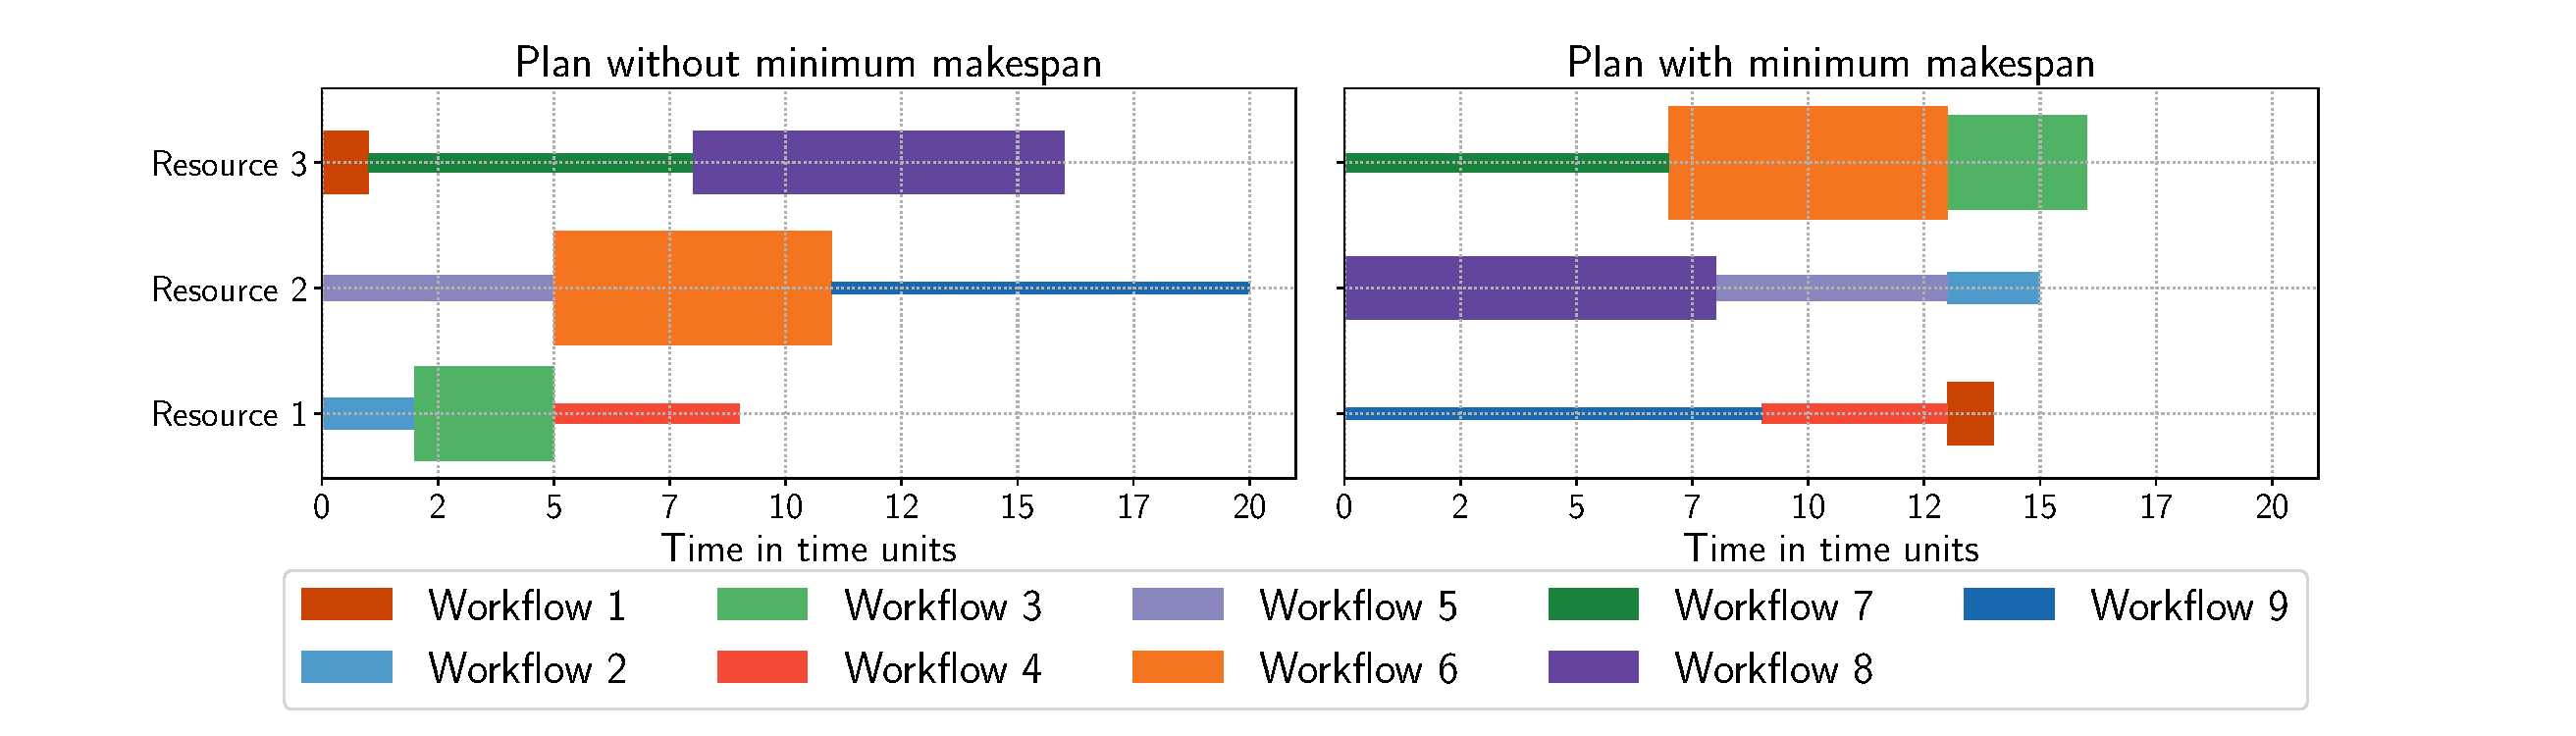
\includegraphics[width=.95\textwidth]{./figures/random_vs_specific.pdf}
    \caption{Comparison of different campaign execution plans. Based on workflow mapping on resources makespan and resource utilization is different.}\label{fig:example_makespan}
\end{figure*}

We are making a set of assumptions which we do not relax during the initial analysis of a model that calculates the makespan of a campaign.
These are:
\begin{inparaenum}[(1)]
    \item a workflow is an atomic unit and cannot be decomposed;
    \item workflow resource request is sufficient to execute the workflow; % and the requested resources are utilized;
    \item a resource is an aggregate of computing capabilities;
    \item resources are homogeneous;
    \item every workflow of a given campaign can be executed on the given resources;
    \item a random resource selection is based on a uniform distribution;
    \item only one workflow can be executed on a resource at any point in time; and
    \item a workflows can be homogeneous or heterogeneous in space---maximum number of resources they need, and time---the amount of time they are executing.
\end{inparaenum}

We denote a computational campaign as $C = [w_{i}: 1 \leq i \leq N_{C}]$, where $w_{i}$ is a workflow and $N_{C}$ is the total number of workflows, $R = [ r_{j}: 1 \leq j \leq N_{R}]$ is a set of available resources, where $r_{j}$ is a resource and $N_{R}$ is the total number of available resources, and $ M(C,R) = [(w_i, r_j): 1 \leq i \leq N_{C}, r_j \in R] $ is a mapping function of workflows onto resources.
In addition, we denote the execution time of a workflow as $Tx_{w_{i}}$, the makespan of campaign $C$ as $TTX_{C}$, and the makespan of campaign $C$ for a given mapping function $ M $ as $TTX_{C}(M)$.
Assumption~\#3 allows to abstract the resource implementation details, as workflows can be executed on different resources such as HPCs, Clouds, pilots and more. 
Lastly, we will assume homogeneous resources as it simplifies the formalization of the problem.

With a single resource, i.e., $N_{R} = 1$, the workflows of a campaign will be executed sequentially, regardless the execution order or if the workflows are homogeneous or heterogeneous.
As a result the makespan of the campaign is:
\begin{equation}
   TTX_{C} = \sum_{i=1}^{N_{C}}Tx_{w_{i}} 
\end{equation}

With multiple homogeneous resources, i.e., $1 < N_{R} < N_{C}$, the workflows of a campaign can be executed concurrently.
Furthermore, this is semantically equivalent to executing on a single resource large enough to allow concurrent workflow execution, where each workflow executes on a resource partition. 
Because of assumptions~\#5 and~\#7, executing homogeneous or heterogeneous in space workflows has the same makespan.
A random mapping of workflows onto resource will have a makespan:
\begin{equation}
   TTX_{C}(Random) \geq \frac{1}{N_{R}}\sum_{i=1}^{N_{C}} Tx_{w_{i}} 
\end{equation}
Given multiple homogeneous resources, when executing workflows that are heterogeneous in time and that can be homogeneous or heterogeneous in space, the makespan of the campaign for a given mapping function $ M $ is:
\begin{equation}
TTX_{C}(M) = \max_{r_{j}\in R}\Big\{\sum_{w_{i}\in M(C,r_{j})}Tx_{w_{i}}\Big\}
\label{eq:makespan}
\end{equation}
\section{Makespan algorithms}
\label{sec:algo}

\section{Makespan algorithm performance comparison}
\label{sec:algo_perf_comp}
